%!TEX root = ThesisLKN.tex
\chapter{Background Knowledge} \label{chapter:3}

This chapter introduces the theoretical background of this thesis, which mainly concerns two distinct parts: Bayesian Occupancy Filter (BOF) and Convolutional Neural Network. In Section \ref{sec:bayes_filtering}, we start with introduction to the idea of Bayesian filtering. BOF is naturally introduced in Section \ref{sec:bof}, since it is an extension of Bayesian filtering on occupancy grid for object tracking. To better adapt BOF to human tracking context, Section \ref{sec:bofmp} explains how our human motion model can be seamlessly incorporated into the BOF framework. In Section \ref{sec:cnn}, we firstly introduce the general structure of CNNs, and the state-of-the-art densely connected CNNs (DenseNets) are explained in Section \ref{sec:dense_net}. To exploit the power of DenseNets for networks that produce \textit{pixel-wise} predictions , the fully convolution DenseNets with upsampling path are introduced in Section \ref{sec:fc_dense_net}. In Section \ref{sec:metrics}, different metrics for evaluating the performance of tracking are discussed. The arguments for our choice of metrics used in this thesis are also provided. 

\section{Bayesian Occupancy Filter} 

In a tracking system, the locations of tracked objects are estimated by taking into accounts both incoming measurements from sensor and predictions from last time step. This process is very similar to Bayesian filtering, which is a probabilistic way to \textit{recursively} estimate the state of a dynamic system.

\subsection{Bayesian Filtering} \label{sec:bayes_filtering}

Bayesian filters work in a dynamic system. At any time $t$, the true state $x_t$ of the dynamic system is unobservable. Instead, measurements $z_t$ can be obtained from sensor data and their relationship can be expresses as \citep{jazwinski2007stochastic}:

\begin{equation}
z_t = h_t(x_t, \omega_t)
\end{equation}

where $h_t$ is normally given in this context and called as \textit{observation model}, $\omega_t$ is known as \textit{measurement noise}. The true state $x_t$ evolves from last state $x_{t-1}$ based on a \textit{process model} $f_t$:

\begin{equation}
x_t = f_t(x_{t-1}, v_{t-1})
\end{equation}

where variable $v_{t}$ is called as \textit{process noise}. This equation describes a \textit{Markov process} with order one, since current state $x_t$ does not depend on past states of $x_{1:t-2}$ and only depends on last state $x_{t-1}$. For a dynamic system, the goal of Bayesian filtering is to recursively estimate the \textit{posterior} probability distribution, $P(x_t|z_{1:t})$. This is done in two steps: \textit{prediction} and \textit{estimation}. In the prediction step, a \textit{prior} distribution on the state of the system is calculated based on posterior distribution from last time step and the process model. In the estimation step, the prior distribution is used with new measurements to calculate  posterior distribution on the current state.

\subsection{BOFUM Formulation} \label{sec:bof}

BOF, similar to Bayesian filer, consists of two stages of \textit{prediction} and \textit{estimation}. Bayesian Occupancy Filter (BOF) can be applied on robots to reason about the dynamic environment, which in this context is represented by occupancy grid. Applications of BOF include collision avoidance \citep{coue2006bayesian} and object tracking \citep{chen2006dynamic}.

Historically, based on different representations of the cell's state space, there are two formulations of BOF: 4D-BOF and 2D-BOF. In 4D-BOF, each cell has four dimensions, with two dimensions representing its position on the gird, and the other two representing the orthogonal velocity components \citep{coue2006bayesian}. While for 2D-BOF, cells are organized as in a 2-dimensional occupancy grid, and each cell is associated with probability distributions of its velocity. The advantage of 4D-BOF is that it is able to represent overlapping objects with different velocities. However, 4D-BOF is more computationally expensive and it is not able to estimate cell's velocity. On the contrary, 2D-BOF dose not allow overlapping objects but requires less computations and is able to infer velocities. In this thesis, we follow the 2D-BOF formulation as proposed by \citet{gindele2009bayesian}, which extends original 2D-BOF using prior map knowledge (BOFUM) as an indicator of motion preference. 			

We start the formulation of BOFUM by introducing relevant random variables. The subscript $n$ of each random variable represents the cell index on the grid map. We assume there are $N$ cells in total. For time step $t$, we define:

\begin{my_enumerate}
\item[] $O:$ Vector for occupancy state of all cells. Each element $O_n$ takes two possible values, $occ$ and $nocc$.
\[ O = (O_1, \ ... \ , \ O_N)^T \in \{ occ, nocc\}^n \]

\item[] $V:$ Vector for velocities in $x$ and $y$ directions. Velocities are discretized into cells, which have unit of $cells/timestep$.
\[ V = (V_1, \ ... \ , \ V_N)^T \in \{ \mathbb{Z}, \mathbb{Z}\}^n \]

\item[] $X:$ Combination of both occupancy and velocity. 
\[ X = (O, \ V) \]

\item[] $X^-:$ Occupancy and velocity state at time $t-1$.
\[ X^- = (O^-, \ V^-) \]

\item[] $R:$ Matrix of random variables describing reachability from cell $a$ to cell $c$. This information is hand-crafted based on cell's context on the grid map. 
\[ R \in \{reach, nreach\}^{n \times n}\]

\item[] $T$: Transition vector. For $T_i = j$, it represents that the occupancy in cell $i$ will move to cell $j$ in the next time step. The transition is an abstraction over velocity, reachability and any other information about the cell movement. 
\[ T = (T_1, \ ... \ , \ T_N)^T \in N^n\]

\item[] $Z$: Measurement vector that comes from sensor data.
\[Z = (Z_O, \ Z_V), Z_O \in  \{ occ, nocc\}^n , Z_V \in \{ \mathbb{Z}, \mathbb{Z}\}^n\]

In our context, we use no sensors for measuring velocities. Therefore, $Z_v$ will be omitted.
\end{my_enumerate}

We assume that cells are independent to each other. This simplifies the formulation and also makes the implementation of BOF highly parallelisable. The goal of BOF is to estimate the posterior probability distribution of the state of a specific cell $c$ given measurement $Z$:
\begin{align}
P(X_c|Z_c) &= \frac{P(X_c, Z_c)}{P(Z_c)} \label{eq:1} \\ 
         &= \frac{\sum_{X^-, R, T}{P(X_c, X^-, R, T, Z_c)}}{\sum_{X^-, R, T, X_c}{P(X_c, X^-, R, T, Z_c)}} 
\end{align}
Since $P(Z_c)$ can be obtained by marginalization, i.e., $P(Z_c)= \sum_{X_c}{P(X_c, Z_c)}$, we only concern the numerator of Equation \ref{eq:1}:
\begin{equation}
P(X_c|Z_c) \propto \sum_{X^-, R, T}{P(X_c, X^-, R, T, Z_c)} \label{eq:4}
\end{equation}

In order to calculate joint probability $P(X_c, X^-, R, T, Z_c)$, we need to decompose it based on Baye's rules and some assumptions. 
\begin{align}
P(X_c, X^-, R, T, Z_c) &= P(X_c, X^-, R, T)P(Z_c|X_c, X^-, R, T) \label{eq:3}\\
                     &= P(X_c, X^-, R, T)P(Z_c|X_c) \\
                     &= \underbrace{P(X_c | X^-, R, T) P(X^-, R, T)}_{prediction} \underbrace{P(Z_c|X_c)}_{correction} \label{eq:2}
\end{align}

So far, the two main stages of Bayesian filtering can been identified by Equation \ref{eq:2}: 

\begin{my_enumerate}
\item \textbf{prediction}: The prediction step calculates a prior distribution of the state of cell $X_c$, which is joint distributed with past state $X^-$, reachability $R$ and transition $T$. It can be further decomposed as in Equation \ref{eq:2}. 

$P(X_c | X^-, R, T)$ specifies the \textit{process model}, which states how the current state can be predicted given a prior state and extra knowledge. Since occupancy and velocity are independent and transition subsumes velocity and reachability, we have
\begin{equation}
P(X_c | X^-, R, T) = P(O_c|O^-, T)P(V_c|O^-, T)
\end{equation}
For the propagation of occupancy, we assume that it is sufficient for a cell $c$ to be occupied, if at least one antecedent cell $a$ moves to cell $c$. This assumption can be expressed as:
\begin{align}
P(O_c=occ|O^-, T) &= 
  \begin{cases}
  1, & \vee_{a \in N} ((O_a=occ) \wedge (T_a=c)) \\
  0, & else
  \end{cases} 
\end{align}
For simplicity of implementation, we calculate `$nocc$' instead of calculating `$occ$':
\begin{align}
P(O_c=occ|O^-, T) &= 1 - P(O_c=nocc|O^-,T) \\
                  &= \prod_{a \in N}{(1-P(O_c=occ|O^-_a,T_a))}
\end{align}
where 
\begin{equation}
P(O_c=occ|O^-_a, T_a) =
  \begin{cases}
  1, & (O_a=occ) \wedge (T_a=c) \\
  0, & else
  \end{cases} 
\end{equation}

For an antecedent cell $a$ that moves to cell $c$, the propagation of velocity is expressed as:
\begin{equation}
P(V_c=v(a, c)| O^-, T) = P(O_c=occ|O^-_a, T_a) \label{eq:6}
\end{equation}
where $v$ is helper function that expresses velocity from cell $a$ to cell $c$.

$P(X^-, R, T)$ is the joint distribution for transition. By assuming occupancy and transition are independent, we have
\begin{align}
P(X^-, R, T) &= P(O^-, V^-, R, T) \\
             &= \prod_{i \in N} P(O_i^-) \prod_{j \in N} P(T_j, V^-, R)
\end{align}
Since we assume \textit{Occupancy preservation}, occupancy of an antecedent cell $a$ must propagate to follower cells m. This introduces a normalization coefficient $\mu$:
\begin{align}
P(T_a=c, V^-, R) &= \frac{P(T_a=c, V^-_a, R_{a,c})}{\sum_{m \in N}P(T_a=m, V^-_a, R_{a,m})} \\
                 &= \mu_a P(V_a^-) P(R_{a,c})P(T_a=c|V_a^-, R_{a, c}) \label{eq:t}
\end{align}
where 
\begin{equation}
P(T_a=c|V^-_a, R_{a,c}) =
  \begin{cases}
  1, & V_a^- = v(a, c) \wedge (R_{a,c} = reach) \\
  0, & else
  \end{cases} 
  \label{eq:t1}
\end{equation}

\item \textbf{estimation}: The estimation step multiplies a prior distribution calculated from \textit{prediction} with a conditional probability distribution that represents \textit{correction} based on an \textit{observation model}. We do not use any sensor for measuring velocity, and we assume cell's occupancy state can be extracted from raw sensor data after preprocessing. The observation model captures the uncertainty involved in sensor measuring given cell's occupancy state:
\begin{align}
P(Z_{O,c}=z_c|X_C) &= P(Z_{O,c}=z_c|O_C) \\
				   &=
				   \begin{cases}
				   1-\omega_Z, & z_c = o_c \\
				   \omega_Z,   & else
				   \end{cases}
\end{align}
where $\omega_Z \in [0,1]$ and higher its value, more confident we are in measurements. 
\end{my_enumerate}

\begin{figure}[ht]
  \centering
    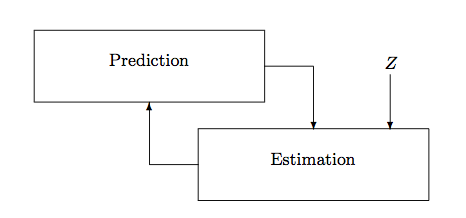
\includegraphics[width=.6\textwidth]{figures/bof_recursive.png}
    \caption[The prediction and estimation loop of BOF.]{The prediction and estimation loop of BOF \citep{tay2008bayesian}}
    \label{fig:bof_recursive}
\end{figure} 

To summarize, the \textit{prediction} and \textit{estimation} steps of BOF work recursively as shown in Figure \ref{fig:bof_recursive}. To calculate posterior probability distribution $P(X_c|Z_c)$, we need firstly calculate the joint distribution in Equation \ref{eq:4} as:
\begin{align}
\sum_{X^-, R, T}P(X_c, X^-, R, T, Z_c) &= P(Z_c|O_c) \sum_{O^-, V^-, R, T}P(V^-,R,T)P(O^-)P(O_c|O^-,T)P(V_c|O^-,T) \notag  \\
                        &= P(Z_c|O_c) \sum_{O^-, T}P(T)P(O^-)P(O_c|O^-,T)P(V_c|O^-,T) \notag \\
                        &=  \underbrace{P(Z_c|O_c)}_{correction} \notag \\
                        & \ \ \ \ \underbrace{\sum_{O^-, T}P(T)P(O^-)P(O_c|O^-,T)}_{occupancy \ prediction} \label{eq:occ_pred} \\
                        & \ \ \ \ \underbrace{\sum_{O^-, T}P(T)P(O^-)P(V_c|O^-,T)}_{velocity  \  prediction} \label{eq:vel_pred}
\end{align}

As can be seen from above equations, $P(T)$ is needed for prediction. Based on Equation \ref{eq:t} and \ref{eq:t1}, we have:
\begin{align}
P(T_a = c) &= \sum_{V^-, R}{\mu_a P(V_a^-)P(R_{a,c})P(T_a=c|V_a^-, R_{a,c})} \\
		   &= \mu_a P(V_a^-=v(a,c))P(R_{a,c}=reach)
\end{align}

Based on Equation \ref{eq:6} and \ref{eq:vel_pred}, velocity prediction can be derived as:
\begin{align}
P(\hat{V_c}=v(a, c)) &= \sum_{O^-, T}P(T)P(O^-)P(\hat{V_c}=v(a,c)|O^-,T) \\
  &= P(O_a^-=occ)P(T_a=c) \label{eq:infer_velocity}
\end{align}

We then apply uncertainty in acceleration on the predicted velocity $\hat{V}$. The acceleration noise is assumed to be normal distribution with zero mean and covariance $\Sigma$. Therefore the final velocity is predicted as:
\begin{equation}
P(V_c) = \sum_{\hat{V_c}}{P(V_c|\hat{V_c})P(\hat{V_c})} \label{eq:adding_noise}
\end{equation}
where
\begin{equation}
v_c = \hat{v_c} + \omega_a \Delta t, \ \omega_a \sim \mathcal{N}(0, \Sigma) \label{eq:adding_noise}
\end{equation}

For occupancy prediction, the probability of a cell being \textit{not} occupied is firstly calculated. It is easier to calculate since only one case needs to be considered, namely when all possible antecedent cells do not move to that cell.
\begin{align}
P(O_c=nocc) &= \sum_{O^-, T} P(O^-)P(T)P(O_c=nocc|O^-,T) \\
            &= \sum_{O^-, T}\prod_{a \in N} P(O_a^-)P(T_a)P(O_c=nocc|O^-_a,T_a) \\
            &= \prod_{a \in N} \sum_{O_a^-, T_a} P(O_a^-)P(T_a)P(O_c=nocc|O^-_a,T_a) \\
            &= \prod_{a \in N} (1-P(O_a^-=occ)P(T_a=c))
\end{align}
Therefore, the probability of a cell being occupied can be calculated as:
\begin{align}
P(O_c=occ) &= 1 - P(O_c=nocc) \\
           &= 1 - \prod_{a \in N}{(1-P(O_a^-=occ)P(T_a=c))}
\end{align}

\subsection{BOF with Motion Pattern (BOFMP)} \label{sec:bofmp}

In the above formulation of BOFUM, if occupancy propagates from an antecedent cell $a$ to cell $c$ with velocity $v(a,c)$, cell $c$ will propagate the occupancy with the same velocity $v(a,c)$ along with zero-mean acceleration noise. In other words, BOFUM assumes a constant velocity motion model with uncertain zero-acceleration. In reality, object actually follows some motion patterns based on its location on the map. For example, a car driving on a lane are more likely to drive along the lane instead of driving to sidewalks. Therefore, \citet{gindele2009bayesian} incorporate this motion preference into the reachability matrix $R$.

For a cell $c$ on the occupancy gird, they assign a terrain type for each cell with a helper function $u$. In their automotive application, they define three terrain types: $U=\{lane, sidewalks, unknown\}$. The reachability probability between cell $a$ and cell $c$ can be calculated as:
\begin{equation}
P(R_{a,c}=reach) = S_{u(a), u(c)} \omega(a, c) \label{eq:reachability}
\end{equation}
where matrix $S\in[0,1]^{U\times U}$ defines the likelihood of change terrain types, and $\omega: N \times N \rightarrow [0,1]$ captures the likelihood of the movement when both cells are in the same terrain type or when the distance between these two cells has influence on the likelihood.

However, their way of modeling place dependent motion patterns has two disadvantages: 1) Manually classifying terrain types might be reasonable in their automotive applications, but it is not feasible in our human tracking scenarios. Although indoor environment, like offices and factories, can be classified as \textit{walkable} or \textit{not walkable}, this kind of classification does not provide too much information on motion preference. 2) As shown in Equation \ref{eq:reachability}, the $S$ matrix and weight function $\omega$ have to be manually defined. When an object is being tracked, the environment is updated rapidly, which requires to update the reachability matrix at the same time. Besides, when large maps are considered, it requires a lot of manual work to define function $\omega$ since any two cells on the grid map have to be considered. Therefore, defining reachability is very time consuming and inflexible. 

To deal with the mentioned disadvantages, we propose to model motion patterns in a \textit{learning-based} way. Although we apply this method only on modeling human motion patterns in indoor environment, it can be also used in other scenarios, such as modeling car motion pattern in outdoor environment. The idea is to train a neural network based on relevant data extracted from human trajectories. Once the network finished training, it learns the implicit motion patterns that are imposed on the human trajectories used for training. For a given gird map, the network is able to output data that can be interpreted as motion patterns without human intervention. This facilitates its application on real scenarios even in rapidly changing environments.   

The relevant data we extracted from human trajectories can be used as an proxy of human motion patterns. They are represented as a set of conditional probabilities for every cell on the map. They represent how likely a person moves to one of the neighboring cells (exit direction), conditioned on which neighboring cell he or she comes from (entering direction). Mathematically, for any cell $c \in [1,N]$ on the gird map, they can be expressed as
\begin{equation}
P_c(V^{ex}|V^{en}) 
\end{equation}
where $V^{ex}, V^{en}$ represent exit and entering direction respectively, and $V^{ex}, V^{en} \in \{U, L, R, D, DL, DR, UL, UR\}$ \footnote{U: up, L: left, R:right, D:down}.
Since these probabilities incorporate information about the incoming cell, the motion model captures \textit{spatial correlations} between cells. Besides, they are different for each cell based on cell’s context on the map, which means the learned motion pattern is expressive enough to predict different motions at different locations. In other words, our motion model is also \textit{place dependent}.

Figure \ref{fig:condi_prob_example} shows an example of how our model captures motion preference based on its location on the map. A person is currently at the location indicated by the green rectangle and arrives by taking entering direction of left. The most possible exit directions, as shown by red arrows in the left plot, show that this person is likely going either up-left or down-left in the next time step. This is expected since we can infer no bias towards either of the directions from the symmetric map. The motion model for the cell related to that location is represented by conditional probabilities shown in the right plot. It only shows $P_c(V^{ex}|V^{en}=L)$.
\begin{figure}[ht]
  \centering
    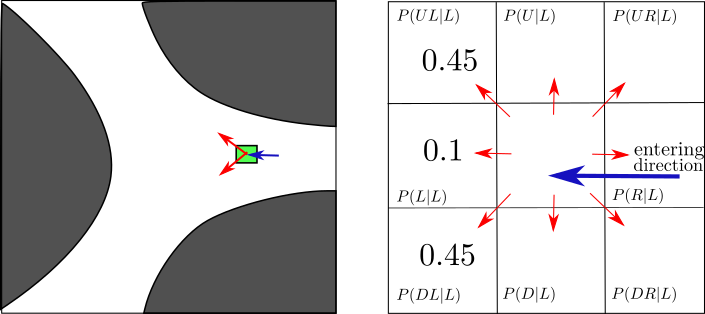
\includegraphics[width=.85\textwidth]{figures/bofmp_example.png}
    \caption[An example of our proposed motion model.]{An example of our proposed motion model. \textbf{LEFT}: A person is at location indicated by green rectangle. White area is walkable. The green arrow and red arrows show entering and exit directions. \textbf{RIGHT}: The motion pattern at that cell represented as $P_c(V^{ex}|V^{en}=L)$. It shows that, for the next time step, this person is more likely to turn either up-left or down-left than keep its entering direction of going left.}
    \label{fig:condi_prob_example}
\end{figure}

The way how we incorporate our motion model into BOFUM similar to adding acceleration noise to predicted velocity in Equation \ref{eq:adding_noise}. After the inferred velocity $\hat{V}$ is calculated based on process model as shown in Equation \ref{eq:infer_velocity}, the final velocity is calculated as:
\begin{equation}
P(V_c) = \sum_{\hat{V_c}}{P_c(V^{ex}=V_c|V^{en}=\hat{V_c})P(\hat{V_c})} \label{eq:motion_pattern}
\end{equation}
where $P_c(V^{ex}|V^{en})$ is \textit{cell-specific} motion pattern. In this ways, the BOFMP knows how to propagate occupancies according to human motion pattern at certain locations. When compared with BOFUM, this method leads to better tracking performance especially when no observations are given or in occluded scenarios.

In this section, we assume the maximum velocity of the object is 1 $cell/timestep$. In reality, the objects may perform higher velocities. However, our neural network that extracts motion patterns models only velocity of 1 $cell/timestep$. The method of how we adapt our motion model to higher velocities will be explained in Section \ref{sec:BOFMP_implementation}.

\section{Convolutional Neural Network} \label{sec:cnn}

Neural networks are mathematical abstraction about how our human nervous system process and learn from data. Over the last few years, neural networks have been extensively used in many applications, such as computer vision \citep{russakovsky2015imagenet}, natural language processing \citep{cho2014learning} and robotics \citep{levine2016learning}. Neural networks are organized as a layered structure, which replicates forward flow of information through human nervous system. Each layer consists of a certain number of \textit{neurons}. In regular neural networks, those layers are \textit{fully} connected. That is, neurons between two adjacent layers are pairwise connected, but neurons within a single layer have no connections with each other. For a single neuron, assuming its inputs are expressed by a vector $\mathbf{x}$, its parameters are weights $\mathbf{w}$ and bias $b$, and its output is a scalar value:
\begin{equation}
y = f(\mathbf{w}^T \mathbf{x} + b)
\end{equation}
where $f$ is a non-linear function, which is known as \textit{activation function}. Popular choices for activation function include:

\begin{my_enumerate}
\item \textbf{Sigmoid function}: $f(x)=\frac{1}{1+e^{-x}} \in [0, 1]$. One undesired property of sigmoid function is that it gets saturated at both ends, which means the gradient for very small or very large inputs are almost zeros. In other words, sigmoid function ``kills'' gradient which may affect training of networks. 
\item \textbf{Tanh function}: $f(x)=\frac{e^x-e^{-x}}{e^x+e^{-x}} \in [-1, 1]$ Similar to sigmoid function, tanh function also saturates and ``kills'' gradients. However, its output is zero-centered.
\item \textbf{ReLU}: $f(x)=max(0, x) \in [0, +\infty)$. ReLU never saturates and this may accelerate convergence of network training as shown in \cite{krizhevsky2012imagenet}. Variants of ReLU include leaky-ReLU and PReLU \cite{he2015delving}.
\end{my_enumerate}

To train a neural network, ground truth must be given since neural network is a supervised learning algorithm. Besides, a \textit{loss function} has to be defined in order to measure how close are our network predictions to the ground truth. Commonly used loss functions are cross-entropy loss for classification and L2 squared norm for regression. Based on the loss calculated for training data, the network has to be optimized in terms of finding the best parameters of the network so that the loss is minimized. It turns out that following the (reversed) direction of gradients of the loss function is an effective way to update these parameters. Based on this observation, many optimization algorithms for neural networks have been proposed, such as Stochastic Gradient Descent (SGD), RMSProp and Adam (see more in \cite{ruder2016overview}). 

Convolutional Neural Networks (CNNs) are a special kind of neural network that works well with image data. In regular neural networks, the neurons for each layer is organized as a one-dimensional vector. While for CNNs, they are arranged in three dimensions: width, height and depth. For the input layer (i.e, the first layer), width and height are the spatial dimensions of an image and depth corresponds to the RGB channels of a color image. For image classification, the output layer is $1\times1\times N$ dimensional, with N corresponding to number of classes. CNNs are also organized as a stack of layers, and the most common layers are:

\begin{my_enumerate}
\item \textbf{Convolutional Layer} (CONV): The core layer of a CNN. CNNs learn the complex structure in image data by firstly extracting useful features, such as edges or a blotch of some color in shallow layers and semantic wheel-like or nose-like features in deeper layers. Those features are extracted by applying filters on 3D volume of data on each layer and this process is represented by a CONV layer. CONV layer utilizes \textit{local connectivity}, which means they extract feature only on a local region of the input data. Thanks to its \textit{parameter sharing} scheme, the number of parameters in CONV layers are much less than in layers of a regular neural network. The output volume of CONV layer depends on three hyperparameters: depth, stride and zero-padding.
\item \textbf{ReLU Layer} (RELU): This layer introduces non-linearities to the network and work as activation function as in regular neural networks. It applies ReLU function point-wise on the input volume.
\item \textbf{Pooling Layer} (POOL): This layer works as a downsampling operation that reduces the size of input data and ensures spatial invariance to some degrees. Typical pooling operation include max pooling and average pooling.
\item \textbf{Fully-connected Layer} (FC): As its name indicated, each of the neuron in FC layer is connected to all neurons in its preceding layer as in regular neural networks. For image classification tasks, the last layer is normally a FC layer. 
\item \textbf{Batch-Normalization Layer}(BN): Batch normalization is a technique that has been proposed in \citep{ioffe2015batch} to address the so-called internal covariate shift phenomena in network training. Using BN layers allows higher learning rate and makes network less sensitive to initialization. 
\end{my_enumerate}

As an example, a simple CNN that used for image classification can be expressed as:
\begin{equation*}
\text{INPUT}\rightarrow[\text{CONV}\rightarrow \text{BN} \rightarrow \text{RELU} \rightarrow \text{POOL}] * 2 \rightarrow \text{FC}
\end{equation*}

\subsection{Densely Connected Convolutional Networks } \label{sec:dense_net}

In the development of CNNs, \citet{Simonyan14c} show that the depth of CNNs plays an very important role in its performance. However, the experiments from \citet{he2016deep} show that with increased depth, the accuracy of network predictions firstly gets saturated and then degrades rapidly. In theory, the deeper network should perform at least as good as its shallower counterpart, because the redundant layers can at least learn an identity mapping, i.e., directly produce input as output. This unexpected performance degradation leads to their conclusion that CNNs are not good at learning identify mapping. To address this problem, they propose \textit{residual} learning. Assume the underlying desired mapping that represented by few stacked layers is $\mathcal{H}(\mathbf{x})$. Instead of learning it directly, its residual,
\[\mathcal{F}(\mathbf{x}) = \mathcal{H}(\mathbf{x}) - \mathbf{x}\]
is learned and a \textit{skip connection} is connected from the input to the output of these stacked layers. Therefore, the final learned mapping is $\mathcal{F}(\mathbf{x}) + \mathbf{x} = \mathcal{H}(\mathbf{x})$. This idea is illustrated in Figure \ref{fig:res_idea}. 
\begin{figure}[ht]
  \centering
    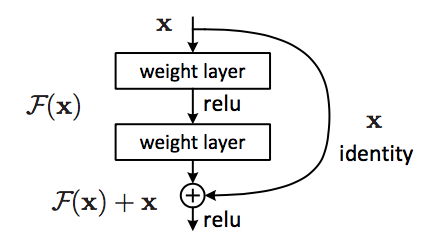
\includegraphics[width=.55\textwidth]{figures/res_idea.png}
    \caption[An illustration of residual learning]{An illustration of residual learning \citep{he2016deep}. Instead of fitting the desired underlying mapping directly, a residual mapping $\mathcal{F}(\mathbf{x})$ is learned with few stacked layers.}
    \label{fig:res_idea}
\end{figure}

The advantages of residual learning is that it facilitates the gradient flow from deep layers to shallow layers through the skip connection. We define a composite function $H_l(\cdot)$ that can be represented by a few stacked layers such as BN, POOL, RELU and CONV. $l$ is the layer index. Therefore, for the input $\mathbf{x}_{l-1}$, the output of residual learning from layer $l$ is:
\begin{equation}
\mathbf{x}_{l} = H_l(\mathbf{x}_{l-1}) + \mathbf{x}_{l-1}
\end{equation}
\citet{huang2016densely} propose a similar network structure that heavily uses skip connections. To encourage \textit{feature reuse}, they concatenate feature maps from all preceding layers $0, \ldots, l-1$, which are then used as input of current layer $l$:
\begin{equation}
\mathbf{x}_{l} = H_l([\mathbf{x}_{0}, \mathbf{x}_{1}, \ldots, \mathbf{x}_{l-1}]) 
\end{equation}

A block of $L$ layers that are densely connected in such a way is called as a \textit{dense block}, and it has $\frac{L(L+1)}{2}$ connections. On example of a five layer dense block is shown in Figure \ref{fig:dense_net}. This special design of DenseNet leads to its state-of-the-art performance in image classification tasks.

\subsection{Fully Convolutional DenseNet} \label{sec:fc_dense_net}

The regular CNN are designed for image classification, where only one vector of class scores is needed from network output. In some other tasks such as semantic segmentation, every pixed has to be classified into a certain class, i.e., the output must have the same spatial resolution as input image. This cannot be achieved by regular CNNs, since pooling operations are essential in networks but they also reduce spatial extent.

To achieve classification at pixel level, fully convolutional neural networks (FCNs) have been proposed by \citet{jegou2017one}. By using only convolutional layers and \textit{deconvolution} layers that functions as upsampling, their network is able to take arbitrary size image as input and predicts pixel-wise classification. A deconvolution operation is essentially \textit{backward} convolution. Deconvolution, compared with interpolation, is a natural choice for upsampling in CNNs since it is learnable and thus facilitates end-to-end learning of the networks. How downsampling and upsampling is achieved in CNNs is illustrated in Figure \ref{fig:sampling}

\begin{figure}[ht]
  \centering
    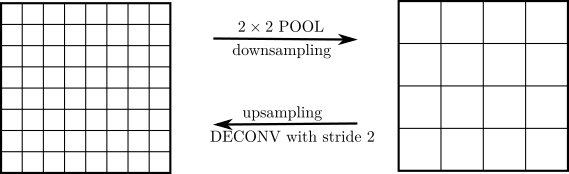
\includegraphics[width=.75\textwidth]{figures/sampling.png}
    \caption[Downsampling and upsampling in FCNs.]{Downsampling and upsampling in FCNs. Left represents a data volume with spatial size of $8\times8$. Downsampling with $2\times2$ pooling operation reduces its size to $4\times4$. Upsamping with deconvolution of stride 2 resumes its size.}
    \label{fig:sampling}
\end{figure}

\citet{jegou2017one} extends fully convolutional networks with dense blocks. Their proposed structure has a downsampling path extracting high-level semantic feature and an upsampling path recovering outputs to full resolution as input image. Their network structure, with some modifications, is used in thesis to extract motion patterns from static maps. As described in Section \ref{sec:bofmp}, we represent motion patterns as cell-specific conditional probabilities $P_c(V^{ex}|V^{en})$. Instead of predicting classification scores, the last layer of our network predicts $8\times8=64$ entries, which are interpreted as eight conditional probability distributions $P_c(V^{ex}|V^{en}=v)$. Each of these conditional probability distributions corresponds to one of eight entering directions. 
